%ChapterV.tex
\section{数字信号的基带传输}\label{chapter:V}
\HyperBack{chapter:V}

    本章及下一章主要研究二进制序列通过数值调制器后在信道中传输并进行解调的基本理论,
    本章是基于基带的调制和基带信道,下一章则是频带信号与频带信道。

\subsection{数字系统的指标}

    数字信源与模拟信源最大的区别是\emph{幅值离散、时间离散}。
    
    \paragraph{信息量的单位}\mbox{}

    如果离散信源是由"0" 、"1"两个符号构成集合,而且输出的二进制序列中
    这两个符号出现概率相等且各符号之间统计独立,则每个符号的信息量为
    \begin{equation}
        I=P_1\log_2\frac{1}{P_1}+P_2\log_2\frac{1}{P_2}=\frac{1}{2}+\frac{1}{2}=1~\text{bit}
    \end{equation}
    若不满足上述条件,即不等概率出现或符号间相关的情况下,每个符号携带的信息量小于1个比特。

    \paragraph{信息传输速率}\mbox{}

    在二进制数字通信系统中每秒传送的二进制符号数可以用每秒传送的最大信息量来表征,
    单位为比特每秒(bit/s)。对于二进制系统,若符号间隔为$T_b$(s),
    每个符号携带的信息为1 bit ,故信息传输速率为$R_b=\dfrac{1}{T_b}$。

    \paragraph{码元传输速率}\mbox{}

    对于$M$\footnote{因为这里的$M$是一个变量,所以要用斜体,笔者:虽然就是加两个\$但也感觉有点麻烦...有的时候还要考虑因为M的右斜要不要补充间距。}
    进制的数字通信系统,每秒传送的$M$的进制符号数被称为码元传输速率或符号速率,单位为波特(Baud),简写Bd,或symbol/s。

    通常$M$是2的整数次幂,即$M=2^K$,表示着每$K$个二进制符号与$M$进制符号之一相对应,则$M$进制符号速率(码元速率)$R_s$
    与二进制信息速率$R_b$的转换关系为
    \begin{equation}
        R_s=\frac{R_b}{\displaystyle\log_2M}=\frac{R_b}{K}\hspace{1em}\text{(Baud)}
    \end{equation}

    \paragraph{误比特率与误符号率}\mbox{}

    误比特率,BER\footnote{龙老师:就一个音节别给我拼成[bɜː]!}(Symbol Error Ratio)与误符号率,SER(Symbol Error Ratio)。
    对于$M$进制的数字通信系统中,误符号率是在符号间隔$T_s$内,发送端发出$M$进制符号$s_i$,经过传输后,结束端接收到的信号$\hat s$不为$s_i$的概率,
    用$P\left(\hat s\neq s_i\mid s_i\right)$表示。当$M=2$的时候,符号退化为比特,即误比特率。

    \paragraph{频带利用率}\mbox{}

    数字通信传输系统的频带利用率定义为:所传输的信息速率(或符号速率)与系统带宽的比值,其单位为bit/s/Hz,而Hz本身就是/s,故单位相当于bit。

\subsection{数字基带信号的波形及其功率谱密度}
    数字脉冲调制有三种基本方法:
    \begin{enumerate}[itemsep=0pt,parsep=0em,label=\color{bupt}\arabic*、,labelsep=0pt,leftmargin=4em]
        \item 脉冲幅度调制(PAM)信号
        \item 脉冲位置调制(PPM)信号
        \item 脉冲宽度调制(PDM)信号
    \end{enumerate}
    由于幅度调制的频带利用率高,故本章只考虑PAM。

    \subsubsection{M-ary PAM信号原理}
    $M$PMA是将不同取值的符号映射为相同的波形函数,仅幅度不同。过程是先将输入的序列
    $\displaystyle\sum_{n=-\infty}^{\infty}a_b\delta(t-nT_b)$进行2/$M$进制转换,
    变为冲击序列$\displaystyle\sum_{n=-\infty}^{\infty}a_n\delta(t-nT_s)$,对于$M=2^K$有$T_s=KT_b$,
    通过发送滤波器变为$s(t)=\displaystyle\sum_{n=-\infty}^{\infty}a_ng_T(t-nT_s)$。

    这里的幅度$a_n$的选取控制着码型,比如对于二进制信号$M=2$,
    选取$a_n\in\{\pm 1\}$或者$a_n\in\{0,1\}$就是两种不同的码型。
    
    \subsubsection{常用的数字PAM信号波形/码型极其功率谱}
    \emph{这一部分的定义和波形主要见书上80--84页,笔记只作为补充\footnote{其实是技术力不够没办法把波形迅速做成矢量图于是就传球了。}}
    
    这里给出对于$s(t)=\displaystyle\sum_{n=-\infty}^{\infty}a_ng_T(t-nT_s)$的一般化的功率谱表达。
    设发送滤波器$g_T(t)\leftrightarrow G_T(f)$,信号$s(t)$的功率谱密度为\footnote{千万不要忘记系数$1/T_s$}
    \begin{equation}\label{eq:PAM-Pf}
        P_s(f)=\frac{1}{T_s}\sum_{k=-\infty}^{\infty}R_a(k)e^{j2\pi kT_sf}\abs{G_T(f)}^2
    \end{equation}

    对于i.i.d.二进制信源,每个符号相互独立,而且各符号等概率出现。

    当$k=0$时
    \begin{equation}
        R_a(k)=\mathscr{E}[a_n^2]=\sigma_a^2+m_a^2
    \end{equation}

    当$k\neq 0$时
    \begin{equation}
        R_a(k)=\mathscr{E}[a_na_{n+k}]\mathscr{E}[a_n]\mathscr{E}[a_{n+k}]=m_a^2
    \end{equation}

    那么
    \begin{equation}\label{eq:idd-PAM-Pf}
        \begin{split}
            P_s(f)&=\frac{\sigma_a^2}{T_s}\abs{G_T(f)}^2+\frac{m_a^2}{T_s}\abs{G_T(f)}^2\sum_{k=-\infty}^{\infty}e^{j2\pi kT_sf}\\
                  &=\underbrace{\frac{\sigma_a^2}{T_s}\abs{G_T(f)}^2}_{\text{连续谱}}+\underbrace{\frac{m_a^2}{T_s^2}\sum_{n=-\infty}^{\infty}\abs{G_T\left(\frac{n}{T_s}\right)}^2\delta\left(f-\frac{n}{T_s}\right)}_{\text{离散的周期谱线}}
        \end{split}
    \end{equation}
    而我们主要关注功率谱如下几方面:
    \begin{enumerate}[itemsep=0pt,parsep=0em,label=\color{bupt}\arabic*、,labelsep=0pt,leftmargin=4em]
        \item 调制信号的带宽
        \item 有无直流分量
        \item 有无定时分量等
    \end{enumerate}
    
    %第二点实际上说明了信号是否有无用的功率消耗在了直流上,我们希望的是在一个较短时间内,总可以做到均值接近于零。

    %第三点在实际应用中可以把周期(定时)的分量滤波出来用作抽样。

    \begin{table}[H]
        \centering
        \caption{六种基本码型的对比}
        \begin{tabular}{c|c|c|c}
            \Xhline{1pt}
            \textcolor{bupt}{码型} & \textcolor{bupt}{主瓣宽度} & \textcolor{bupt}{直流分量} & \textcolor{bupt}{定时分量}\\ \Xhline{0.5pt}
            \textcolor{bupt}{单极不归零码} & $R_b$ & 有 & 无      \\ \Xhline{0.5pt}
            \textcolor{bupt}{双极不归零码} & $R_b$ & 无 & 无      \\ \Xhline{0.5pt}
            \textcolor{bupt}{单极归零码}   & $2R_b$ & 有 & 有     \\ \Xhline{0.5pt}
            \textcolor{bupt}{双极归零码}   & $2R_b$ & 无 & 无     \\ \Xhline{0.5pt}
            \textcolor{bupt}{差分码}      & $R_b$  & \multicolumn{2}{c}{取决于码型} \\ \Xhline{0.5pt} 
            \textcolor{bupt}{$M$PAM}     & $R_s$ & 无 & 无 \\ \Xhline{1pt}
        \end{tabular}
    \end{table}

    举一道应用的例题,书上\emph{[例题5.2.10]}:

    二进制信息序列$\{b_n\}$的取值为$+1$或$-1$,出现概率相等且符间不相关。
    由其经前后算数加运算得到的前后相关序列$\{a_n\}$,
    \begin{equation}
        a_n=b_n+b_{n-1}\hspace{1em}\text{(算数加)}
    \end{equation}
    若发送滤波器冲激响应$g_T(t)$为矩形不归零脉冲,请写出由此发送的PAM信号$s(t)$的功率谱。

    \paragraph{方法一}:

    \vspace{-2ex}
    \begin{equation}
        m_a=\mathscr{E}[a_n]=\mathscr{E}[b_n+b_{n-1}]=0\hspace{0.8em}
    \end{equation}
    \vspace{-6ex}
    \begin{equation}
        \begin{split}
            R_a(k)  &=\mathscr{E}[a_na_{n+k}]\\
                    &=\mathscr{E}[(b_n+b_{n-1})(b_{n+k}+b_{n+k-1})]\\
                    &=\begin{cases}
                        2\hspace{2em}m=0\\
                        1\hspace{2em}m=\pm 1\\
                        0\hspace{2em}\text{else}
                    \end{cases}
        \end{split}
    \end{equation}
    发送滤波器的冲激响应为
    \begin{equation}
        g_T(s)=\text{rect}\left[\frac{1}{T_b}(t-\frac{T_b}{2})\right]\xleftrightarrow[]{\mathscr{F}}T_b\text{sinc}\left(T_bf\right)e^{-j2\pi f\frac{T_b}{2}}
    \end{equation}
    带入\eqaref{eq:PAM-Pf}得,
    \begin{equation}
        \begin{split}
            P_s(f)  &=\frac{1}{T_s}\sum_{k=-\infty}^{\infty}R_a(k)e^{j2\pi kT_sf}\abs{G_T(f)}^2\\
                    &=\frac{1}{T_b}(e^{-j2\pi T_bf}+2+e^{j2\pi T_bf})\abs{T_b\text{sinc}\left(T_bf\right)e^{-j2\pi f\frac{T_b}{2}}}^2\\
                    &=2T_b[1+\cos(2\pi T_bf)]\text{sinc}^2\left(T_bf\right)\\
                    &=4T_b\cos^2(\pi T_bf)\text{sinc}^2\left(T_bf\right)
        \end{split}
    \end{equation}

    \paragraph{方法二}:

    将原系统视作由i.i.d数字信源$\{b_n\}$产生的信号通过发送滤波器后,再通过冲激响应为
    $h(t)=\delta(t)+\delta(t-T_b)$的线性时不变系统。
    由\eqaref{eq:idd-PAM-Pf}得通过发送滤波器后的信号的功率谱为
    \begin{equation}
        \begin{split}
            P_{s'}(f)   &=\frac{1}{T_b}\abs{T_b\text{sinc}\left(T_bf\right)e^{-j2\pi f\frac{T_b}{2}}}^2\\
                        &=T_b\text{sinc}^2\left(T_bf\right)
        \end{split}
    \end{equation}

    $h(t)$的功率谱为
    \begin{equation}
        P_h(f)=\abs{1+e^{-j2\pi fT_b}}^2=e^{-j2\pi T_bf}+2+e^{j2\pi T_bf}=4\cos^2(\pi T_bf)
    \end{equation}
    总的输出信号的功率谱为
    \begin{equation}
        P_s(f)=P_{s'}(f)P_h(f)=4T_b\cos^2(\pi T_bf)\text{sinc}^2\left(T_bf\right)
    \end{equation}

    \paragraph{方法三}\footnote{实际上这个方法对于更一般的情况,要比前两个情况的计算更复杂。但是对于本题,两个冲激响应平移后拼接而成的新的冲激响应恰好有一个简单的形式,故便于计算。}:

    沿用上一方法思路,但把$g_T(t)$和$h(t)$视作一个系统。总的冲激响应为
    \begin{equation}
        \begin{split}
            g_{T'}(t)&=g_T(t)*h(t)\\
                     &=\text{rect}\left[\frac{1}{T_b}(t-\frac{T_b}{2})\right]+\text{rect}\left[\frac{1}{T_b}(t-\frac{T_b}{2}+T_b)\right]\\
                     &=\text{rect}\left[\frac{1}{2T_b}(t-T_b)\right]
        \end{split}
    \end{equation}
    其功率谱为
    \begin{equation}
        P_{T'}(f)=\abs{2T_b\text{sinc}(2T_bf)e^{-j2\pi fT_b}}^2=4T_b^2\text{sinc}^2(2T_bf)
    \end{equation}
    再由\eqaref{eq:idd-PAM-Pf}得
    \begin{equation}
        \begin{split}
            P_s(f)  &=\frac{1}{T_b}4T_b^2\text{sinc}^2(2T_bf)\\
                    &=4T_b\frac{\sin^2(2\pi T_bf)}{(2\pi T_bf)^2}\\
                    &=4T_b\frac{4\sin^2(\pi T_bf)\cos^2(\pi T_bf)}{4(\pi T_bf)^2}\\
                    &=4T_b\cos^2(\pi T_bf)\text{sinc}^2\left(T_bf\right)
        \end{split}
    \end{equation}

    \subsubsection{常用线路码型}
    线路码型的设计应遵守以下原则
    \begin{enumerate}[itemsep=0pt,parsep=0em,label=\color{bupt}\arabic*、,labelsep=0pt,leftmargin=4em]
        \item 线路码的功率谱特性与基带信道的频率特性相匹配:无直流分量,减少低频分量。
        \item 减少线路码频谱中的高频分量:节省频带,不产生\hyperref[subsubsec:ISI]{ISI}。
        \item 便于符号同步信号提取:线路码频谱特性不受信源的统计特性影响;对用户透明,不限制用户的使用。
        \item 减少误码扩散。
        \item 便于误码检测。
        \item 尽量提高编码效率。
    \end{enumerate}

    \paragraph{AMI码:传号交替反转码}\mbox{}

    AMI是一种三元码, “1”交替的变换为“+1”和“-1”, “0”保持不变。每个码型都是归零码, 脉冲宽度为符号\emph{宽度的一半}。

    其优点
    \begin{enumerate}[itemsep=0pt,parsep=0em,label=\color{bupt}\arabic*、,labelsep=0pt,leftmargin=4em]
        \item 无直流;高频、低频分量小。
        \item 全波整流后即为单极性RZ码,可提取定时信息。
        \item 具有检错能力,根据极性的交替性可以做出判断。
    \end{enumerate}

    其缺点
    \begin{enumerate}[itemsep=0pt,parsep=0em,label=\color{bupt}\arabic*、,labelsep=0pt,leftmargin=4em]
        \item 功率谱特性与信源特性密切相关。
        \item 连0多时,AMI整流后连0也多,不利于提取高质量的位同步信号。
    \end{enumerate}

    例:
    \begin{table}[H]
        \centering
        \begin{tabular}{c|*{19}{c}c}
            \textcolor{bupt}{$b_n$} &1 &0 &1 &1 &0 &0 &0 &0 &0 &0 &0 &1 &1 &0 &0 &0 &0 &0 &0 &1 \\ \Xhline{0.3pt}
            \textcolor{bupt}{$a_n$} &+1 &0 &-1 &+1 &0 &0 &0 &0 &0 &0 &0 &-1 &+1 &0 &0 &0 &0 &0 &0 &-1
        \end{tabular}
    \end{table}

    \paragraph{HDB3码:三阶高密度双极性码}\mbox{}

    其特点为“1”交替变换为“+1”和“-1”的半占空归零码,连“0”数不超过3。
    编码规则为
    \begin{enumerate}[itemsep=0pt,parsep=0em,label=\color{bupt}\arabic*、,labelsep=0pt,leftmargin=4em]
        \item 先变为AMI码, 将连“0”按每4个一组进行划分, 并将4个连“0”用“000V”或“B00V”取代。
        \item V的极性与前一个非零符号保持一致, B与前一个非0码极性相反。\footnote{实际上说明BV是同极性}
        \item 相邻V满足极性交替反转特性: 相邻V之间有奇数个非0时用“000V”,否则用“B00V”。
        \item B符号后的非0符号从V符号开始再交替反转极性。
    \end{enumerate}
    其中B代表Balance,保持极性交替规则:与前非0符号极性相反。
    V代表Violence,破坏极性交替规则:与前非0符号极性相同。
    
    其保持了AMI码的优点;改善了长连0问题,定时提取方便,但直流特性较AMI稍差一点(毕竟V破坏了交替性)。
    \emph{与AMI一样,虽然为归零码元,但其交替性使得其频谱主瓣宽度与非归零码一样,都是$R_b$,而且分布在低频\footnote{工作在低频容易受到50Hz的市电干扰。}和高频分布较少。}
    具体图见书上92页图5.2.17。

    例1:
    \begin{table}[H]
        \centering
        \begin{tabular}{c|*{19}{c}c}
            \textcolor{bupt}{\hspace{-3pt}$b_n$\hspace{-3pt}} &1 &0 &1 &1 &0 &0 &0 &0 &0 &0 &0 &1 &1 &0 &0 &0 &0 &0 &0 &1 \\ \Xhline{0.3pt}
            \textcolor{bupt}{\hspace{-3pt}$AMI$\hspace{-3pt}} &+1 &0 &-1 &+1 &\textcolor{pur}{0} &\textcolor{pur}{0} &\textcolor{pur}{0} &\textcolor{pur}{0} &0 &0 &0 &-1 &+1 &\textcolor{pur}{0} &\textcolor{pur}{0} &\textcolor{pur}{0} &\textcolor{pur}{0} &0 &0 &-1 \\ \Xhline{0.3pt}
            \textcolor{bupt}{} &+1 &0 &-1 &+1 &\textcolor{pur}{?} &\textcolor{pur}{0} &\textcolor{pur}{0} &\textcolor{pur}{+V} &0 &0 &0 &-1 &+1 &\textcolor{pur}{?} &\textcolor{pur}{0} &\textcolor{pur}{0} &\textcolor{pur}{-V} &0 &0 &-1 \\ \Xhline{0.3pt}
            \textcolor{bupt}{\hspace{-3pt}HDB${}_3$\hspace{-3pt}} &+1 &0 &-1 &+1 &\textcolor{pur}{0} &\textcolor{pur}{0} &\textcolor{pur}{0} &\textcolor{pur}{+V} &0 &0 &0 &-1 &+1 &\textcolor{pur}{-B} &\textcolor{pur}{0} &\textcolor{pur}{0} &\textcolor{pur}{-V} &0 &0 &\textcolor{red}{+1} \\\Xhline{0.3pt}
            \textcolor{bupt}{}&+1 &0 &-1 &+1 &0 &0 &0 &+1 &0 &0 &0 &-1 &+1 &-1 &0 &0 &-1 &0 &0 &+1
        \end{tabular}
    \end{table}

    其译码相对比较简单,每个破坏极性交替的即是V,将其与前3个替换为0并全波整流即可:
    \begin{table}[H]
        \centering
        \begin{tabular}{c|*{19}{c}c}
            \textcolor{bupt}{HDB${}_3$\hspace{-2pt}} &+1 &0 &-1 &+1 &0 &0 &0 &\textcolor{red}{+1} &0 &0 &0 &-1 &+1 &-1 &0 &0 &\textcolor{red}{-1} &0 &0 &+1 \\ \Xhline{0.3pt}
            {}&+1 &0 &-1 &+1 &\textcolor{pur}{0} &\textcolor{pur}{0} &\textcolor{pur}{0} &\textcolor{pur}{0} &0 &0 &0 &-1 &+1 &\textcolor{pur}{0} &\textcolor{pur}{0} &\textcolor{pur}{0} &\textcolor{pur}{0} &0 &0 &+1 \\ \Xhline{0.3pt}
            \textcolor{bupt}{$b_n$\hspace{-2pt}} &1 &0 &1 &1 &0 &0 &0 &0 &0 &0 &0 &1 &1 &0 &0 &0 &0 &0 &0 &1
        \end{tabular}
    \end{table}

    \paragraph{nBmB码}\mbox{}

    是把原信息码流的n位二进制码作为一组,变换为m位二进制码作为新的码组。

    如下文的双相码、Miller码、CMI码都是1B2B码;光纤数字传输系统则用到5B6B码;ASCII则是一种7B8B码,为7bit + 1CRC。

    \paragraph{CMI (coded mark inversion)码:传号反转码}\mbox{}

    把“1”交替用11和00, “0”用01来表示。具有检错能力;有较多的电平跃变,定时信息丰富。

    \paragraph{双相码/分相码/Manchester码}\mbox{}

    曼切斯特码把“1”用10表示, “0”用01表示,频谱中含有丰富的定时信息,严格\emph{无直流漂移},但功率谱的主瓣宽度比AMI、HDB3功率谱的主瓣宽一倍。

    用于Ether网、红外通信、RFID、NFC等系统中的线路传输码型。

    \paragraph{Miller码:延迟调制码}\mbox{}

    密勒码把“1”用10或01表示,“1”码元起始不跃变,中心点出现跃变来表示;
    “0”用00或11表示:单个“0”时,保持0前的电平不变,即码元边界及码元中间点电平不跃变。
    连续 “0”,则使连续两个“0”的边界处发生电平跃变。

    双相码的下降沿对应Miller码的跃变沿,频谱主瓣宽度仍为$2R_b$。常用于磁记录接口, RFID。

    例;
    \begin{table}[H]
        \centering
        \begin{tabular}{c|*{8}{c}}
            \textcolor{bupt}{$b_n$} & 1 & 1 & 0 & 1 & 0 & 0 & 1 & 0 \\ \Xhline{0.3pt}
            \textcolor{bupt}{双相码} & 10 & 10 & 01 & 10 & 01 & 01 & 10 & 01 \\ \Xhline{0.3pt}
            \textcolor{bupt}{密勒码} & 01 & 10 & 00 & 01 & 11 & 00 & 01 & 11
        \end{tabular}
    \end{table}

\subsection[AWGN下的数字基带信号的接收]{在加性高斯白噪声信道条件下数字基带信号的接收}
    在此信道模型中,认为发送的PAM数字基带信号\footnote{在本节中只考虑}
    与随机噪声是相加的,即接收的信号
    \begin{equation*}
        r(t)=s_i(t)+n_w(t)\hspace{2em}i=1\text{或}2,0\leq t\leq T_b
    \end{equation*}

    其中$n_w(t)$的功率谱为$P(f)=\dfrac{N_0}{2}$。
    \subsubsection{利用匹配滤波器的最佳接收}

    确定信号在受到AWGN的干扰下的最佳接收是采用\hyperref[subsec:matched-filter]{匹配滤波器},使得在
    \emph{最佳采样时刻}的信噪比最大,然后选择合适的判决门限进行判决,可以使平均误比特率最小。

    对于$s(t)=\displaystyle\sum_{n=-\infty}^{\infty}a_ng_T(t-nT_s)$,在$0\leq t\leq T_b$时,
    \vspace{-2ex}
    \begin{equation}
        s(t)=\begin{cases}
            a_1g_T(t)\\
            a_2g_T(t)
        \end{cases}
    \end{equation}

    最佳接收时刻为$t_0=T_b$的匹配滤波器的单位冲激响应为
    \begin{equation}
        h(t)=K\cdot g_T(T_b-t) 
    \end{equation}

    不妨设$K=1$,那么最佳接收时刻接收到的信号中有用信号的值为$a_iE_g,i=1,2$。
    其中$E_g$是$g_T(t)$的能量;而噪声的功率则为$\dfrac{N_0}{2}E_g$。
    那么此时接收的的信号可以写成
    \begin{equation}
        y(T_b)=a_iE_g+Z\sim\mathscr{N}\left(a_iE_g,\sqrt{\frac{N_0}{2}E_g}\right)
    \end{equation}

    判决器为
    \vspace{-2ex}
    \begin{equation}
        \hat{s}(t)=\begin{cases}
            a_1,y(T_b)<V_T\\
            a_2,y(T_b)>V_T
        \end{cases}
    \end{equation}

    对于双极不归零码,$g_T(t)=A,a_1=-1,a_2=1$,每一比特的能量$E_b=E_g=A^2T_b$。
    平均误比特率为
    \begin{equation}
        P_b=P\left(e\mid a_1\right)P(a_1)+P\left(e\mid a_2\right)P(a_2)
    \end{equation}
    可以知道,使误比特率最小的\emph{最佳门限电平}
    \begin{equation}
        V_T=\frac{N_0}{4}\ln\left[\frac{P(a_1)}{P(a_2)}\right]
    \end{equation}
    对于i.i.d信源,则$V_T=0$,误码率
    \begin{equation}\label{eq:BERofBNRZ}
        P_b=\frac{P(a_1)}{2}\text{erfc}\left(\sqrt{\frac{E_b}{N_0}}\right)+\frac{P(a_2)}{2}\text{erfc}\left(\sqrt{\frac{E_b}{N_0}}\right)=\frac{1}{2}\text{erfc}\left(\sqrt{\frac{E_b}{N_0}}\right)
    \end{equation}

    而对于单极不归零码,$g_T(t)=A,a_1=0,a_2=1$,平均每一比特的能量$E_b=A^2T_b/2$。
    使误比特率最小的\emph{最佳门限电平}
    \begin{equation}
        V_T=\frac{E_g}{2}+\frac{N_0}{2}\ln\left[\frac{P(a_1)}{P(a_2)}\right]
    \end{equation}

    对于i.i.d信源,则$V_T=\dfrac{E_g}{2}$,误码率
    \begin{equation}
        P_b=\frac{1}{2}\text{erfc}\left(\sqrt{\frac{E_g}{4N_0}}\right)=\frac{1}{2}\text{erfc}\left(\sqrt{\frac{E_b}{2N_0}}\right)
    \end{equation}

\subsection{PAM信号通过限带信道传输}
    不难知道,时域上有限的信号,频域上是无限宽的;
    相应的,严格限带的信号在时域上也是无线宽的。
    所以对于带限信道,必须设计带限基带信号以使信号能无失真通过信道。

    限带信道可以等效于理想低通滤波器。设其传递函数为$c(t)\xleftrightarrow[]{\mathscr{F}}C(f)$,
    那么从信源到判决器之间的等效信道为
    \begin{equation}
        x(t)=g_T(t)*c(t)*g_R(t)\xleftrightarrow[]{\mathscr{F}}G_T(f)C(f)G_R(f)
    \end{equation}

    那么信源产生的序列$\displaystyle\sum_{n=\infty}^{\infty}a_n\delta(t-nT_s)$,
    判决器在抽样时刻$t=mT_s+t_0$的采样值为
    $\displaystyle\sum_{n=\infty}^{\infty}a_nx(mT_s-nT_s)+\gamma(mT_s)$。
    为使误码率足够小,
    必须最大限度减少ISI(Inter Symbol Interference)和随机噪声($\gamma(t)$)的影响。
    其中后者可以靠匹配滤波器来解决。前者则是接下来推导所讨论的内容。

    \subsubsection{符号间干扰}\label{subsubsec:ISI}
    符号间干扰,ISI(Inter Symbol Interference)。
    对于接收到的信号 
    \begin{equation}
        \sum_{n=\infty}^{\infty}a_nx(mT_s-nT_s)=a_mx(0)+\sum_{m\neq n}a_nx(mT_s-nT_s)
    \end{equation}
    其中$a_mx(0)$为希望接受到的信号,其余的均为符间干扰。

    \subsubsection{无ISI传输的Nyquist准则}
    
    为使接收到的信号码间干扰为零,需满足
    \begin{equation}
        \begin{split}
            x(mT_s-nT_s)=0\hspace{2em}n\neq m\\
            x(mT_s-nT_s)\neq 0\hspace{2em}n= m
        \end{split}
    \end{equation}
    即相当于总的等效的信号的冲激响应满足
    \begin{equation}
        x(nT_s)=\begin{cases}
            1\hspace{2em}n=0\\
            0\hspace{2em}n\neq 0
        \end{cases}
    \end{equation}
    即对于理想抽样有
    \begin{equation}
        \sum_{n=-\infty}^{\infty}x(nT_s)\delta(t-nT_s)=\delta(t)
    \end{equation}
    做如下变形:
    \begin{equation}
        \begin{split}
            \sum_{n=-\infty}^{\infty}x(nT_s)\delta(t-nT_s)&=\delta(t)\\
            x(t)\cdot\sum_{n=-\infty}^{\infty}\delta(t-nT_s)&=\delta(t)\\
            x(t)\frac{1}{T_s}\sum_{m=-\infty}^{\infty}e^{j2\pi \frac{m}{T_s}t}&=\delta(t)\\
            \sum_{m=-\infty}^{\infty}x(t)e^{j2\pi \frac{m}{T_s}t}&=T_s\delta(t)
        \end{split}
    \end{equation}
    上式两侧做傅里叶变换则得到
    \begin{equation}
        \sum_{m=-\infty}^{\infty}X\left(f-\frac{m}{T_s}\right)=T_s
    \end{equation}
    即得到无码间干扰的奈奎斯特准则:
    \begin{mythm}{奈奎斯特准则}\label{thm:Nyquist}
        为使$x(t)$满足
        \begin{equation}
            x(nT_s)=\begin{cases}
                1\hspace{2em}n=0\\
                0\hspace{2em}n\neq 0
            \end{cases}
        \end{equation}
        即无符间干扰,其\emph{充分必要}条件是$x(t)$的傅里叶变换$X(f)$满足
        \begin{equation}
            \sum_{m=-\infty}^{\infty}X\left(f-\frac{m}{T_s}\right)=T_s
        \end{equation}
    \end{mythm}

    根据定理则分为以下情况进行讨论:
    \paragraph{$R_s>2W$}\mbox{}

    在此情况下,$T_s<\dfrac{1}{2W}$,任意两个相邻的$X(f-\dfrac{m}{T_s})$与$X(f-\dfrac{m+1}{T_s})$
    之间没有重叠,必不能满足\hyperref[thm:Nyquist]{奈奎斯特准则}。

    \paragraph{$R_s=2W$}\mbox{}

    在此情况下,称此时的系统带宽$W=\dfrac{1}{2T_s}$为\emph{奈奎斯特带宽};
    称此时的符号速率$R_s=2W$为\emph{奈奎斯特速率};
    称此时的符号周期$R_s$为\emph{奈奎斯特间隔};
    此时的频带利用率$\dfrac{R_s}{W}=2$Baud/Hz为\emph{理想极限},
    是系统的最高的频带利用率,但相应的,
    要求此时的传递函数是一个低通滤波器,其物理不可实现。

    假定存在冲激响应为sinc函数的理想低通滤波器,
    由于\emph{拖尾衰减太慢},衰减速度是$\dfrac{1}{t}$的,当采样时间间隔不严格等于$T_s$的时候,
    实际的采样就会存在码间干扰。

    \paragraph{$R_s<2W$}\mbox{}

    此时两个相邻的$X(f-\dfrac{m}{T_s})$与$X(f-\dfrac{m+1}{T_s})$会相互重叠,
    如果想满足\hyperref[thm:Nyquist]{奈奎斯特准则},
    则需要边沿类似于VSB一样对称滚降。

    可以使用升余弦型的滤波器,
    其传递函数为
    \begin{equation}
        X(f)=\begin{cases}
            T_s\hspace{18.5em}0\leq\abs{f}\leq\dfrac{1-\alpha}{2T_s}\\
            \dfrac{T_s}{2}\left\{1+\cos\left[\dfrac{\pi T_s}{\alpha}\left(\abs{f}-\dfrac{1-\alpha}{2T_s}\right)\right]\right\}\hspace{2em}\dfrac{1-\alpha}{2T_s}<\abs{f}\leq\dfrac{1+\alpha}{2T_s}\\
            0\hspace{20.7em}\abs{f}>\dfrac{1+\alpha}{2T_s}
        \end{cases}
    \end{equation}
    对应的冲激响应为
    \begin{equation}
        x(t)=\text{sinc}\left(\frac{\pi t}{T_s}\right)\cdot\frac{\cos\left(\dfrac{\pi \alpha t}{T_s}\right)}{1-4\left(\dfrac{\alpha t}{T_s}\right)^2}
    \end{equation}
    其中$\alpha$为滚降因子,取值为$0\leq\alpha\leq1$。特别的,当$\alpha=0$时,退化为理想低通滤波器;
    当$\alpha=1$时,退化为一个上抬到x轴上方的余弦周期。
    $\alpha$的物理意义是实际的带宽比$\dfrac{1}{T_s}$多出$\alpha$倍。
    一半为了能够在物理上实现,一般要求$\alpha>0.2$。

\subsection{在理想限带信道及AWGN下数字PAM信号的最佳基带传输}
    对于发送滤波器+信道+匹配滤波器的总体的传递函数$X(f)$,
    在上一节已经证明,如果希望没有符间干扰,则需要满足
    \hyperref[thm:Nyquist]{奈奎斯特准则}。
    其中普遍应用的为升序弦滤波器。即
    \begin{equation}
        G_T(f)C(f)G_R(t)=X(f)
    \end{equation}

    为使判决器采样得到的信噪比最小,
    需要让$G_R(f)$是$G_T(f)C(f)$的\hyperref[subsec:matched-filter]{匹配滤波器},
    考虑到理想信道的$C(t)$是理想低通滤波器,
    就有
    \begin{equation}
        G_R(f)=G_T^*(f)\hspace{2em}g_R(t)=g_T(-t)
    \end{equation}

    那么此时就有系统的总体函数为$X(f)=\abs{G_T(f)}^2=\abs{G_R(f)}^2$,
    结合升余弦滤波器则有
    \begin{equation}
        G_T(f)=G_R(f)=\sqrt{X_{\text{升余弦}}(f)}
    \end{equation}

    若使用双极码,则有发送信号的功率谱\footnote{绘图时应当注意,不同于前面的基于方波的码型,升余弦信号的频谱严格带限。}
    \begin{equation}
        P_s(f)=\frac{\sigma_a^2}{T_s}X_{\text{升余弦}}(f)
    \end{equation}

    举一道例题:某基带系统的信道为理想信道,带宽为2000Hz,今欲以$M$PAM方式传输速率为6000bit/s的数据。
    需满足:(i)进制数M尽量低; (ii)滚降系数α不低于0.25。请给出这个最佳基带传输系统的设计。

    通常来讲,\emph{$M$是2的整数次幂}

    (1)$M=2$。此时系统的符号速率$R_s=R_b=6$k Baud/s,其奈奎斯特带宽为3kHz,大于信道的2kHz,不存在满足要求且无符间干扰的传输系统。

    (2)$M=4$。此时系统的符号速率$R_s=\dfrac{R_b}{\log_2M}=3$k Baud/s,其奈奎斯特带宽为1.5kHz。
    为充分利用信道,取$\alpha=\dfrac{1}{3}$的升余弦,即为符合题意的最佳基带传输系统。

    (3)$M=8$。此时系统的符号速率$R_s=\dfrac{R_b}{\log_2M}=2$k Baud/s,其奈奎斯特带宽为1kHz。
    为充分利用信道,取$\alpha=1$的升余弦,该设计仍然合理,但$M$不是最小的结果。

\subsection{眼图}
    眼图实际是上十一整数个信号周期为宽度在示波器上对输入的PAM信号进行扫描。
    每个周期的波形受到噪声的干扰并相互重叠,产生了类似于人眼的形状,称为眼图。
    从眼图中可以获取如下信息:
    \begin{enumerate}[itemsep=0pt,parsep=0em,label=\color{bupt}\arabic*、,labelsep=0pt,leftmargin=4em]
        \item 进制数$M$为眼数减一。
        \item 眼睛张开的程度反应噪声容限。
        \item 眼睛张开最大的时刻也是最佳采样时刻。
        \item 眼图斜边的斜率决定了系统的噪声容限,越陡峭对定时误差越敏感。
        \item 当码间干扰十分严重的时候,眼睛会接近闭合,此时系统无码严重。
    \end{enumerate}

\subsection{信道均衡}
    因为一般信道的传递函数并不是理想低通滤波器,
    为了仍能理用奈奎斯特准则降低码间干扰,
    故在\emph{接收滤波器}后边串接一个信道均衡器。
    
    \paragraph{线性均衡器}\mbox{}

    如书上\emph{107页图5.7.2},线性均衡器是一个FIR滤波器。
    使用了2N个延迟单元,2N+1个抽头,以及一个加法器构成。
    输入信号经过延迟单元之后,分别和抽头系数$w_n$相乘并求和(加权平均)。

    关于系数$w_n$的计算一是以最小峰值畸变为准则的\emph{迫零算法},
    一个是以最小均方误差为准则的\emph{均方误差算法}。

    前者可以参考\emph{书上108页}。
    其缺点为没有考虑到信道上的加性高斯白噪,矩阵接近奇异矩阵的时候,
    可能会导致噪声被急剧放大。故可以引出平衡符间干扰和噪声的均方误差算法。

\subsection{部分相应系统}
    在无符间干扰一节中,我们给出了利用升余弦滤波器来实现无符间干扰的的设计。
    但是因为其带宽超过奈奎斯特带宽,降低了频带利用率。

    所以在本节中使用了相关编码,人为引入\emph{可以解码的}符间干扰,
    以改变频谱形状,在可实现的同时满足奈奎斯特带宽。

    这里直接使用$\alpha=0$的升余弦滤波器,即带宽为$\dfrac{R_s}{2}$的低通滤波器。
    但在发送滤波器和电平转换之间接入一个相关编码器,其单位冲激响应为
    $h(t)=\delta(t)+\delta(t-T_b)$,其功率谱为$P_h(f)=4 cos2(\pi T_bf)$。
    
    通过滤波器后,总的传递函数
    \begin{equation}
        X_1(f)=\begin{cases}
            2\cos(\pi f T_b)e^{-j\pi f T_b}\hspace{1em}\abs{f}\leq\dfrac{1}{2T_b}\\
            0\hspace{9em}f\text{为其他值}
        \end{cases}
    \end{equation}
    对应的单位冲激响应为
    \begin{equation}
        h(t)=\frac{\sin\left(\dfrac{\pi t}{T_b}\right)}{\dfrac{\pi t}{T_b}}+\frac{\sin\dfrac{\pi (t-T_b)}{T_b}}{\dfrac{\pi (t-T_b)}{T_b}}=\frac{T_b^2\sin\dfrac{\pi t}{T_b}}{\pi t(T_b-t)}
    \end{equation}

    \begin{figure}[H]
        \centering
        \subcaptionbox*{(a)频域}[200pt][c]{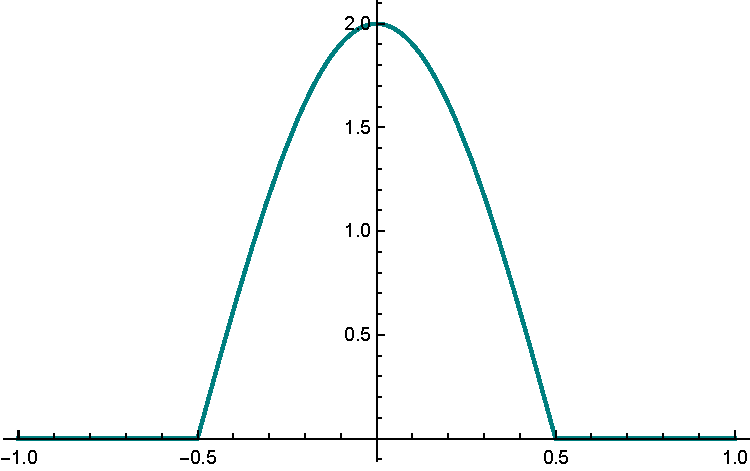
\includegraphics[scale=0.5]{body/image/book582.pdf}}
        \hspace{3em}
        \subcaptionbox*{(b)时域}[200pt][c]{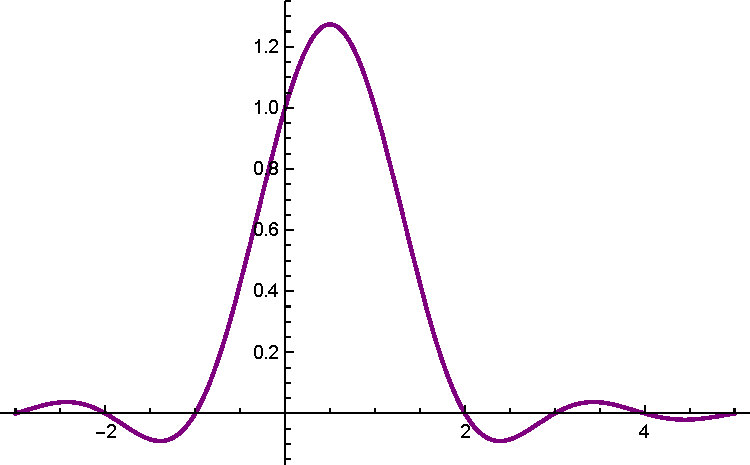
\includegraphics[scale=0.5]{body/image/book583.pdf}}
        \caption{第一类部分相应系统的时频域特性}
    \end{figure}

    可见其在保证了物理可实现性的同时,加快了拖尾衰减速度,其衰减近似与$\dfrac{1}{t^2}$成正比。

    接收的到的信号经过判决器后,得到接收到的序列$\{c_n\}$,恢复$\{a_n\}$的方法则为相关编码的反运算:
    \begin{equation}
        \hat{a}_n=c_n-\hat{a}_{n-1}
    \end{equation}
    但是这种方法有一缺点,当出现一个误码之后,后边的一串码都会出现错误,这种现象称之为\emph{误码传播}。
    
    为了解决这个这个缺点,可以将原码使用预编码进行处理。系统结构见书上\emph{116页图5.8.4},
    预编码器定义为
    \begin{equation}
        d_n=b_n\oplus d_{n-1}
    \end{equation}
    即差分编码。

    不难推导出,当采样输出$c_n=\pm 2$时,判决为0;当采样输出$c_n=0$时,判决为1。

    例:
    \begin{table}[H]
        \centering
        \begin{tabular}{ll|*{13}{r}}
            \textcolor{bupt}{输入数据}  & $\{b_n\}$       &  & 1& 1& 1& 0& 0& 1& 0& 1& 1& 1& 0& 0\\ \Xhline{0.3pt}
            \textcolor{bupt}{预编码输出}& $\{d_n\}$       & 0& 1& 0& 1& 1& 1& 0& 0& 1& 0& 1& 1& 1\\ \Xhline{0.3pt}
            \textcolor{bupt}{二电平序列}& $\{a_n\}$       &-1&+1&-1&+1&+1&+1&-1&-1&+1&-1&+1&+1&+1\\ \Xhline{0.3pt}
            \textcolor{bupt}{采样序列}  & $\{c_n\}$       &  & 0& 0& 0&+2&+2& 0&-2& 0& 0& 0&+2&+2\\ \Xhline{0.3pt}
            \textcolor{bupt}{判决输出}  & $\{\hat{b}_n\}$ &  & 1& 1& 1& 0& 0& 1& 0& 1& 1& 1& 0& 0
        \end{tabular}
    \end{table}

\subsection{符号同步}
    数字通信系统中,为了能够对接收到的信号进行周期性的采样与判决,
    接收端必须要有一个与收到的数字基带信号的符号速率同步的时钟信号。

    书中提及两个方法

    \paragraph{谱线法}\mbox{}

    将原信号平方(不能是归零码),通过窄带滤波器或者锁相环提取余弦定时信号,
    再将其转化为方波信号作为时钟信号。

    \paragraph{超前-滞后门同步器}

    具体原理见书上\emph{119}页,其核心原理是利用眼图在最佳采样时刻张开最大,且关于最佳采样时刻对称。
    故在采样时刻两侧$\pm\Delta$的时刻也进行采样,比较大小,将当前采样时刻向较大一侧偏移。




